\documentclass[a4paper,11pt]{scrartcl}
\usepackage[utf8x]{inputenc}			
\usepackage[T1]{fontenc}				
\usepackage[english]{babel}			
%\usepackage{ulem}
\usepackage{color}						
\usepackage{amsmath,amstext,amssymb,amsfonts,amsthm,mathrsfs,chemarrow,stackrel,dsfont}   % Math packages
\usepackage{graphicx} 					
\usepackage{subcaption}					
%\usepackage{cite}	
\usepackage[round]{natbib} % Bio citation format

\usepackage{microtype}
\usepackage{array}
\usepackage{booktabs}

\usepackage{lineno}

\usepackage{xr-hyper}
\makeatletter
\newcommand*{\addFileDependency}[1]{% argument=file name and extension
  \typeout{(#1)}
  \@addtofilelist{#1}
  \IfFileExists{#1}{}{\typeout{No file #1.}}
}
\makeatother
 
\newcommand*{\myexternaldocument}[1]{%
    \externaldocument{#1}%
    \addFileDependency{#1.tex}%
    \addFileDependency{#1.aux}%
}

%%% END HELPER CODE ------------------------------------
\myexternaldocument{main} %% add link to the maintext file of your revised manuscript in the file list (new file, from another project). 

\usepackage[pdftex, breaklinks, colorlinks, citecolor=black, urlcolor=black, linkcolor=black]{hyperref} 

%\usepackage{fourier} % FD I try to avoid the default LaTeX font for non math journals
%\usepackage{FiraSans}
% \florence Ah you do not like my typefaces ;-)
\usepackage{soul} % FD to strike out, highlight, ...

% Packages to comment out before submitting!
\usepackage[textsize = scriptsize, backgroundcolor = white, linecolor = black]{todonotes}
\usepackage{showlabels}

%\numberwithin{equation}{section}
%\setlength{\parindent}{0pt}
\allowdisplaybreaks[2]

\newcolumntype{P}[1]{>{\centering\arraybackslash}m{#1}}     % Table formatting
\renewcommand{\arraystretch}{1.1}                           % Table formatting

\definecolor{darkgreen}{rgb}{0.0, 0.42, 0.24}
\definecolor{darkblue}{rgb}{0.0, 0.0, 0.55}
\definecolor{change}{rgb}{0.5,0.,0.6}

%%%%%% our commenting commands
\newcommand{\florence}[1]{\textcolor{purple}{(#1)}} % Changed red to purple
\newcommand{\francois}[1]{\textcolor{darkblue}{(#1)}}
\newcommand{\hildegard}[1]{\textcolor{darkgreen}{(#1)}}
\newcommand{\pete}[1]{\textcolor{orange}{(#1)}}
\newcommand{\chg}[1]{\textcolor{change}{#1}}

%%%%%% Putting an S before the equation, section and figure numbering
\renewcommand\theequation{S\arabic{equation}}
\renewcommand\thesection{S\arabic{section}}
\renewcommand\thefigure{S\arabic{figure}}

%opening
\title{Supplementary Information: ``The effect of habitat choice on evolutionary rescue in subdivided populations''}
\author{Peter Czuppon, Fran\c{c}ois Blanquart, Hildegard Uecker,\\ Florence D\'{e}barre}
\date{\today}

\begin{document}

\maketitle

\tableofcontents
\newpage

%Adjusted line numbers (with S before number) but does not work with the cross-referencing... Edit: cross-referencing does not work because of transitivity! It seems you can only refer to ONE document anyway and not to multiple documents. This means that we need to include the linenumbers of the Supplement by hand anyway. Therefore, I changed the linenumbers to S\linenumber. Edit2: I found an easier solution
%\renewcommand\makeLineNumber{\ifodd\value{linenumber} \else\hss\linenumberfont S\thelinenumber\hskip\linenumbersep \fi}
\renewcommand\thelinenumber{S\arabic{linenumber}}
\linenumbers{}
\modulolinenumbers[2]


%%%%%%%%%%%%%%%%%%%%%%%%%%%%%%%%%%%%%%%%%%%%%%%%%%%%%%%%%
% Model dynamics %%%%%%%%%%%%%%%%%%%%%%%%%%%%%%%%%%%%%%%%
%%%%%%%%%%%%%%%%%%%%%%%%%%%%%%%%%%%%%%%%%%%%%%%%%%%%%%%%%
\section{Deriving the model dynamics}
\linelabel{test}In this section we provide the mathematical \chg{details} of the model that is verbally described in the main text. We start by deriving the population dynamics of the wild type \chg{when alone} in both patch types. This will allow us to compute the local growth rate of the mutant \chg{when rare} in old-habitat patches, $a_{\text{old}}$.  

Before we go into the details of the computation, we recall the form of the dispersal rates. For a wild-type individual to disperse to a new-habitat patch, this probability is given by

\begin{equation}\label{Seq:dispersal_rates_old}
    m_w^{\text{new}} = m\, \frac{1-f_{\text{old}}}{1-f_{\text{old}} + \widehat{\pi}_w f_{\text{old}}}\, ,
\end{equation}
%
with $m$ denoting the emigration probability, $f_{\text{old}}$ the frequency of old-habitat patches and $\widehat{\pi}_w$ the transformed wild-type bias towards old-habitat patches.
Analogously, the probability for a wild-type individual \chg{to emigrate and} to move to an old-habitat patch reads
%
\begin{equation}\label{Seq:dispersal_rate_new}
    m_w^{\text{old}} = m\, \frac{\widehat{\pi}_w f_{\text{old}}}{1-f_{\text{old}} + \widehat{\pi}_w f_{\text{old}}}\, .
\end{equation}
\\

All the subsequent computations can be checked with a symbolic programming language (e.g. \textit{Mathematica}). A \textit{Mathematica} notebook is deposited on Gitlab\footnote{\url{https://gitlab.com/pczuppon/evolutionary\_rescue\_and\_dispersal}}.

\subsection*{Stationary wild-type population sizes}
We derive the (deterministic) stationary population sizes of the wild-type in both patch types. These values are denoted by $\widehat{N}_w^{k}$, where $k$ corresponds to the patch type (old or new). In old-patch habitats we assume that the population is always at its carrying capacity. Therefore, we have $\widehat{N}_w^{\text{old}} = K_{\text{old}}$.

In new-habitat patches, the stationary value is given by the solution of the following equation:

 \begin{equation}\label{Seq:wt_deme2}
	\begin{aligned}
		\widehat{N}_w^{\text{new}} &= \left(1-m + m\frac{(1-f_{\text{old}})}{(1-f_{\text{old}}+\widehat{\pi}_w f_{\text{old}})} \frac{(1-f_{\text{old}})M}{(1-f_{\text{old}})M}\right)(1-r)\widehat{N}_w^{\text{new}} \\
		&\qquad \qquad \qquad \qquad \qquad \qquad \qquad \qquad + m_w^{\text{new}} \frac{f_{\text{old}} M}{(1-f_{\text{old}})M} (1-r)  \widehat{N}_w^{\text{old}}\\
		 &= \left(1-m+m_w^{\text{new}} \right)(1-r)\widehat{N}_w^{\text{new}} + m_w^{\text{new}} \left(\frac{f_{\text{old}}}{1-f_{\text{old}}}\right) (1-r)  K_{\text{old}},
	\end{aligned}
\end{equation}
%
which simplifies to
%
\begin{equation}
	\widehat{N}_w^{\text{new}} = \frac{m (1-r) f_{\text{old}}  K_{\text{old}}}{m f_{\text{old}} \widehat{\pi}_w + r(1-f_{\text{old}}+f_{\text{old}}\widehat{\pi}_w -m \widehat{\pi}_w f_{\text{old}})}\ .
\end{equation}
%
Since we assume density regulation, this value cannot be larger than $K_{\text{new}}$, the carrying capacity of new-habitat patches. Hence, we find
\begin{equation}
	\widehat{N}_w^{\text{new}} =\left\{ \begin{array}{ll} 
		K_{\text{new}}, & \text{if }\frac{m (1-r) f_{\text{old}}  K_{\text{old}}}{m f_{\text{old}} \widehat{\pi}_w + r(1-f_{\text{old}}+f_{\text{old}}\widehat{\pi}_w -m \widehat{\pi}_w f_{\text{old}})}\geq K_{\text{new}}; \\
		\frac{m (1-r) f_{\text{old}} K_{\text{old}}
		}{m f_{\text{old}} \widehat{\pi}_w + r(1-f_{\text{old}}+f_{\text{old}}\widehat{\pi}_w -m \widehat{\pi}_w f_{\text{old}})}, & \text{otherwise}.
	\end{array}\right.
\end{equation} 

\subsection*{Wild-type population sizes after dispersal}
In order to explicitly compute the growth rate of the mutant in old-habitat patches, we need an analytical expression for the number of wild-type individuals after the dispersal step. Later on, in the approximation of the probability of adaptation, we also use the number of wild-type individuals in new-habitat patches before reproduction. We denote these values by $\widetilde{N}_w^k$, where $k$ corresponds to the habitat type (old or new). These are given as the solutions to the following equations

\begin{equation}
	\begin{aligned}
		\widetilde{N}_w^{\text{old}} &= \left(1-m + m\, \frac{\widehat{\pi}_w f_{\text{old}}}{(1-f_{\text{old}}+\widehat{\pi}_w f_{\text{old}})}\,  \frac{f_{\text{old}}M}{f_{\text{old}}M} \right) \widehat{N}_w^{\text{old}} + m_w^{\text{old}} \frac{(1-f_{\text{old}})M}{f_{\text{old}}M}\widehat{N}_w^{\text{new}}\ , \\
		\widetilde{N}_w^{\text{new}} &= \left(1-m + m\frac{(1-f_{\text{old}})}{1-f_{\text{old}}+\pi f_{\text{old}}} \frac{(1-f_{\text{old}})M}{(1-f_{\text{old}})M}\right)\widehat{N}_w^{\text{new}} + m_w^{\text{new}} \frac{f_{\text{old}} M}{(1-f_{\text{old}})M} \widehat{N}_w^{\text{old}}\ .
	\end{aligned}
\end{equation}
Using $\widehat{N}_w^{\text{old}}=K_{\text{old}}$ and in the case of $\widehat{N}_w^{\text{new}} = K_{\text{new}}$ this reduces to
\begin{equation}\label{Seq:wt_eq1}
	\begin{aligned}
		\widetilde{N}_w^{\text{old}} &= \frac{(1-f_{\text{old}})m\widehat{\pi}_w K_{\text{new}} + (1-m-f_{\text{old}}(1-m-\widehat{\pi}_w))K_{\text{old}}}{1-f_{\text{old}}+\widehat{\pi}_w f_{\text{old}}} \\ 
		\widetilde{N}_w^{\text{new}}&= \frac{(1-f_{\text{old}}+f_{\text{old}}\widehat{\pi}_w (1-m))K_{\text{new}} + m f_{\text{old}} K_{\text{old}}}{1-f_{\text{old}}+\widehat{\pi}_w f_{\text{old}}}\ .
	\end{aligned}
\end{equation}
%
If on the other hand $\widehat{N}_w^{\text{new}}<K_{\text{new}}$ holds, we obtain
\begin{equation}\label{Seq:wt_eq2}
	\begin{aligned}
		\widetilde{N}_w^{\text{old}} &= \left(1-m+m_w^{\text{old}} \right)K_{\text{old}}\\
		&\qquad \qquad + \left(m_w^{\text{old}} \frac{m (1-r) f_{\text{old}}}{m f_{\text{old}} \widehat{\pi}_w + r(1-f_{\text{old}}+f_{\text{old}}\widehat{\pi}_w -m \widehat{\pi}_w f_{\text{old}})}\left(\frac{1-f_{\text{old}}}{f_{\text{old}}}\right)\right) K_{\text{old}} \\
		%&= \left(1-m_1+\frac{m_1 m_2 (1-r)}{(1-(1-m_2)(1-r))}\right) K \\ 
		&= \frac{m \widehat{\pi}_w f_{\text{old}} + r (1-m) (1-f_{\text{old}} (1-\widehat{\pi}_w))}{m \widehat{\pi}_w f_{\text{old}} + r (1-f_{\text{old}} + \widehat{\pi}_w f_{\text{old}} (1-m))} K_{\text{old}}\ \\
		&= \left(1 - \frac{r m (1-f_{\text{old}}) }{m \widehat{\pi}_w f_{\text{old}} + r (1-f_{\text{old}} + \widehat{\pi}_w f_{\text{old}} (1-m))} \right) K_{\text{old}}\, ,\\
		\widetilde{N}_w^{\text{new}} &= \left(1-m+m_w^{\text{new}}\right) \frac{m (1-r) f_{\text{old}} }{m f_{\text{old}} \widehat{\pi}_w + r(1-f_{\text{old}}+f_{\text{old}}\widehat{\pi}_w -m \widehat{\pi}_w f_{\text{old}})}\, K_{\text{old}}\\
		&\qquad \qquad \qquad \qquad \qquad \qquad \qquad \qquad \qquad \qquad \qquad + m_w^{\text{new}} \frac{f_{\text{old}}}{(1-f_{\text{old}})} K_{\text{old}}\\
		%&= \left(\frac{(1-m_2) m_1 (1-r) f }{(1-f)(1-\left(1-m_2 \right)(1-r))} + \frac{m_1 f}{(1-f)}\right) K\\
		&= \frac{m f_{\text{old}}}{m \widehat{\pi}_w f_{\text{old}} + r(1- f_{\text{old}} + \widehat{\pi}_w f_{\text{old}}  (1-m)) }\, K_{\text{old}}\, .
	\end{aligned}
\end{equation}

\subsection*{Wild-type population sizes during the environmental change}
\chg{Lastly, compute the (deterministic) wild-type population size over time during the environmental change. This value is used in the approximation of the probability of evolutionary rescue in eq.~\eqref{eq:evol_rescue} in the main text, more precisely to estimate the number of rescue mutants that appear during the deterioration of patches.} 

\chg{If a patch deteriorates its current population size is given by the carrying capacity of the old habitat, $K_{\text{old}}$. Subsequently, it is reduced by $(1-r)$, the fecundity of a single wild-type individual in a new-habitat patch. That is, neglecting dispersal for the moment, in generation $j$ after the degradation of a patch, we would have 
\begin{equation}
    N_w^{\text{new}}(j) = K_{\text{old}}(1-r)^j
\end{equation}
wild-type individuals in this patch. Including dispersal between the patches then results in the following number of wild-type individuals in a patch $i$ at time $j$, given that there are $k-1$ other new-habitat patches
\begin{equation}
    N_w^{i,k}(j) = (1-r)\left((1-m)N_w^{i,k}(j-1) + \frac{m_w^{\text{new}}}{k} (M-k) K_{\text{old}} + \frac{m_w^{\text{new}}}{k} \sum_{l=1}^k N_w^{l,k}(j-1) \right)\ .
\end{equation}
The first term represents the remaining individuals after emigration, $(1-m)$, the second and third term are immigrants from old- and new-habitat patches (distributed equally among the $k$ new-habitat patches), respectively. 
}

\subsection*{The local growth rate $a_{\text{old}}$}
As stated in eq.~\eqref{eq:sold} in the main text, we define the growth rate of a single mutant in the old habitat by
\begin{equation}
    1 + a_{\text{old}} = K_{\text{old}}\, \frac{\omega^\text{old}_m}{\omega^\text{old}_w \widetilde{N}_w^{\text{old}}}\, .    
\end{equation}
%
Having computed the number of wild-type individuals after dispersal in an old-habitat patch, $\widetilde{N}_w^{\text{old}}$, we can write the growth rate as follows

\begin{equation}\label{Seq:s_old}
    a_{\text{old}} = \left\{ \begin{array}{ll}
        \frac{\omega^\text{old}_m K_{\text{old}}}{\omega^\text{old}_w \left(\frac{(1-f_{\text{old}})m\widehat{\pi}_w K_{\text{new}} + (1-m-f_{\text{old}}(1-m-\widehat{\pi}_w))K_{\text{old}}}{1-f_{\text{old}}+\widehat{\pi}_w f_{\text{old}}} \right)}\, - 1 , & \text{if } \widehat{N}_w^{\text{new}} = K_{\text{new}};  \\
        \frac{\omega^\text{old}_m}{\omega^\text{old}_w \left(1 - \frac{rm(1-f_{\text{old}})}{f_{\text{old}}m\widehat{\pi}_w + r(1-f_{\text{old}}+\widehat{\pi}_w f_{\text{old}}(1-m))}\right)}\, - 1 , & \text{otherwise}. 
    \end{array}
    \right.
\end{equation}

\subsection*{The local growth rate $a_{\text{new}}$}
\chg{In new-habitat patches we assume that during the relevant phase of establishment of a rare mutant the carrying capacity $K_{\text{new}}$ is not reached. Then the growth rate of the mutant in these patches, $a_{\text{new}}$, is not affected by the different dispersal schemes.} 

\chg{Of course there may be parameter configurations, typically high emigration rates $m$ and a bias of the wild type towards the new habitat ($\pi_w < 0$), where our assumption of density-independent reproduction is violated. Then our approximation and the numerical solution of eq.~\eqref{eq:ext_prob} in the main text strongly deviate from the simulation results (e.g. the New-New dispersal scheme in Fig.~\ref{fig:vary_m_est}(d)).}

%%%%%%%%%%%%%%%%%%%%%%%%%%%%%%%%%%%%%%%%%%%%%%%%%%%%%%%%%
% Establishment probability %%%%%%%%%%%%%%%%%%%%%%%%%%%%%
%%%%%%%%%%%%%%%%%%%%%%%%%%%%%%%%%%%%%%%%%%%%%%%%%%%%%%%%%
\newpage
\section{Approximation of the establishment probability}
We compute the survival probability \chg{of the lineage} of a single mutant starting either in an old- or in a new-habitat patch. We call this probability the establishment probability because it implies the successful establishment of a mutant population within the meta-population. It is denoted by $\varphi_k$ where the index $k$ indicates the initial habitat type of the mutant (old or new).

Our method is the same as used in \citet{tomasini_2018} with the exception that our growth rate in old-habitat patches, $a_{\text{old}}$, depends on the demography of the population. The method in general is based on the theory of multi-type branching processes, cf.~Chapter~5.5 in \citet{haccou_book}. For a detailed application of the theory we refer to the Supplementary Information of \citet{tomasini_2018}. 

We start by recalling the mean reproduction matrix of a mutant that gives the average number of offspring in a certain habitat, dependent on the habitat type in which the mutant resides. It is given as (see also eq.~\eqref{eq:mean_repro} in the main text)

\begin{equation}\label{Seq:mean_repro}
	\mathcal{M} = \bordermatrix{ ~ & \text{old patch} & \text{new patch} \cr
		\text{old patch} & \left(1-m_m^{\text{new}}\right) (1+a_{\text{old}}) & m_m^{\text{new}} (1+a_{\text{new}}) \cr
		\text{new patch} & m_m^{\text{old}} (1+a_{\text{old}}) & \left(1-m_m^{\text{old}}\right) (1+a_{\text{new}})
		}\ ,
\end{equation}
where the rows denote the parent locations, and the columns the patch type of the offspring.

Our goal is to apply Theorem 5.6 from \citet{haccou_book} which states that for a slightly super-critical branching process, \chg{i.e. where the survival probability is slightly above zero}, the establishment probability can be expressed in terms of the largest eigenvalue $\rho$ and the corresponding left- and right-eigenvectors of the mean reproduction matrix \chg{$\mathcal{M}$}, denoted by $u$ and $v$, respectively. The eigenvectors should be normalized in the following way: $u_1+u_2 = 1$ and $\sum_{i=1}^2 u_i v_i = 1$. The establishment probabilities are then given by 
\begin{equation}\label{Seq:theory}
	\varphi_i = \frac{2(\rho-1)}{B} v_i + O(\varepsilon), 
\end{equation}
with
\begin{equation} 
	B = \sum_{i=1}^2 u_i \sum_{j=1}^2 v_j \mathcal{M}_{ij} + \rho(1-\rho) \sum_{j=1}^2 u_j v_j^2\, . 
\end{equation} 

\subsection*{Computing the largest eigenvalue}
We first approximate the largest eigenvalue of $\mathcal{M}$ denoted by $\rho$. It is given by (see \textit{Mathematica} notebook)
\begin{equation}
\begin{aligned}
    \rho &= \frac{1}{2}\left(2 + a_{\text{old}} + a_{\text{new}} - m -  m_m^{\text{new}} a_{\text{old}} - m_m^{\text{old}} a_{\text{new}} \right.\\
    &\quad \left. + \sqrt{4 (m -1) (1+a_{\text{old}})(1+a_{\text{new}}) + (2+a_{\text{old}} + a_{\text{new}} - m - m_m^{\text{new}} a_{\text{old}} - m_m^{\text{old}} a_{\text{new}}})^2 \right)
\end{aligned}
\end{equation}
%
In order to make analytical progress and to identify under which conditions the process is slightly super-critical, i.e. $\rho>1$, we rescale the parameters by a small parameter $\varepsilon$. We set $a_{\text{old}} = \varepsilon, a_{\text{new}} = \varepsilon \xi$ and $m = \varepsilon\mu$. Assuming that $\varepsilon$ is small enough, i.e. effectively a weak selection assumption in old-habitat patches, we can neglect higher orders of $\varepsilon$ and find
\begin{equation}\label{eq:eigenvalue}
\begin{aligned}
    \rho &\approx 1+\frac{1}{2}\varepsilon\left(1+ \xi - \mu + \sqrt{(\xi -1 + \mu_m^{\text{new}})^2 + 2(1-\xi+\mu_m^{\text{new}})\mu_m^{\text{old}} + (\mu_m^{\text{old}})^2  }\right)\\
    &= 1+\frac{1}{2}\varepsilon\left(1+ \xi - \mu + \sqrt{\frac{\gamma}{1-f_{\text{old}}+\widehat{\pi}_m f_{\text{old}}}  }\right),
\end{aligned}
\end{equation}
where $\gamma$ is the rescaled version of the constant $C$ in the main text (eq.~\eqref{eq:normalization}), i.e.
\begin{equation}
    \gamma = (1-f_{\text{old}})(\xi-1+\mu)^2 + \widehat{\pi}_m f_{\text{old}} (\xi-1-\mu)^2\, .
\end{equation}
%
For $\varepsilon\to 0$ we find that $\rho\to 1$ \chg{(eq.~\eqref{eq:eigenvalue}) which means that the branching is slightly super-critical if $\rho>1$ and real. A sufficient condition for this to be true is}
\begin{equation}
    1+\xi-\mu > 0 \quad \Leftrightarrow \quad a_{\text{old}} + a_{\text{new}} - m > 0
\end{equation}
%
\chg{In case that the branching process is not super-critical the establishment probability in eq.~\eqref{Seq:theory} becomes negative and as such is not a probability anymore. Hence, we can simply reject negative solutions of the establishment probability and by that implicitly justify that our approximation is valid.}%\\

%Inserting $\rho$ into equation~\eqref{eq:theory} we see the the enumerator is of order $\varepsilon$.

\subsection*{Computing the establishment probability}
For the solution of eq.~\eqref{Seq:theory} it remains to compute the normalized eigenvectors. Their precise form is of not much insight. We therefore omit stating them explicitly but refer to the \textit{Mathematica} notebook. Solving eq.~\eqref{Seq:theory} to the first order of $\varepsilon$ we find

\begin{equation}
    \begin{aligned}
        \varphi_{\text{old}} &= \varepsilon + \frac{\varepsilon\left(1-\xi\right)}{\sqrt{\frac{\gamma}{(1-f_{\text{old}}+\widehat{\pi}_m f_{\text{old}})}}}  + \frac{\varepsilon\left(\mu_m^{\text{old}} -\mu_m^{\text{new}} + 2 \mu_m^{\text{new}}\xi  \right)}{\sqrt{\frac{\gamma}{(1-f_{\text{old}}+\widehat{\pi}_m f_{\text{old}})}}}\, ,\\
        \varphi_{\text{new}} &= \varepsilon\xi + \frac{\varepsilon\xi \left(\xi-1\right)}{\sqrt{\frac{\gamma}{(1-f_{\text{old}}+\widehat{\pi}_m f_{\text{old}})}}} + \frac{\varepsilon\left(\xi \mu_m^{\text{new}} -\xi \mu_m^{\text{old}} + 2 \mu_m^{\text{old}}  \right)}{\sqrt{\frac{\gamma}{(1-f_{\text{old}}+\widehat{\pi}_m f_{\text{old}})}}}\, .
    \end{aligned}
\end{equation}
%
Transforming back to the original variables and replacing $\gamma$ by the constant $C$ from the main text (eq.~\eqref{eq:normalization})
\begin{equation}
    C = (1-f_{\text{old}}+\widehat{\pi}_m f_{\text{old}}) \left((1-f_{\text{old}})(a_{\text{new}}-a_{\text{old}}+m)^2 + \widehat{\pi}_m f_{\text{old}} (a_{\text{new}}-a_{\text{old}}-m)^2\right)\, ,
\end{equation}
we obtain

\begin{equation}
    \begin{aligned}
        \varphi_{\text{old}} &= a_{\text{old}} + \frac{(1-f_{\text{old}}+\widehat{\pi}_m f_{\text{old}})a_{\text{old}} \left(a_{\text{old}}-a_{\text{new}}\right)}{\sqrt{C}}  + \\
        &\qquad \qquad \qquad m \frac{\left(\widehat{\pi}_m f_{\text{old}} a_{\text{old}} - (1-f_{\text{old}}) a_{\text{old}} + 2 (1-f_{\text{old}}) a_{\text{new}}  \right)}{\sqrt{C}}\, ,\\
        \varphi_{\text{new}} &= a_{\text{new}} + \frac{(1-f_{\text{old}}+\widehat{\pi}_m f_{\text{old}})a_{\text{new}} \left(a_{\text{new}} - a_{\text{old}}\right)}{\sqrt{C}} \\
        &\qquad \qquad \qquad + m \frac{\left(a_{\text{new}} (1-f_{\text{old}}) - a_{\text{new}} \widehat{\pi}_m f_{\text{old}} + 2 a_{\text{old}} \widehat{\pi}_m f_{\text{old}}  \right)}{\sqrt{C}}\, .
    \end{aligned}
\end{equation}
%
Slightly re-ordering the terms, this gives the establishment probability of a single mutant individual, eq.~\eqref{eq:estab_approx} in the main text:
\begin{equation}\label{Seq:estab_approx}
	\begin{aligned}
		\varphi_{\text{old}} &\approx \qquad \quad \; \; \; \; a_{\text{old}} \qquad \quad \;  \; +  \quad a_{\text{old}} \frac{\left(1-f_{\text{old}}+\widehat{\pi}_m f_{\text{old}}\right)}{\sqrt{C}}(a_{\text{old}}-a_{\text{new}}) \\
		& \qquad \qquad + \frac{m}{\sqrt{C}} \left(a_{\text{new}}(1-f_{\text{old}}) + a_{\text{old}}\widehat{\pi}_m f_{\text{old}} - (a_{\text{old}}-a_{\text{new}})(1-f_{\text{old}})\right) \, ,\\
		\varphi_{\text{new}} &\approx \underbrace{ a_{\text{new}}}_{\text{(1) local growth parameter}} +  \quad \underbrace{ a_{\text{new}} \frac{\left(1-f_{\text{old}}+\widehat{\pi}_m f_{\text{old}}\right)}{\sqrt{C}}(a_{\text{new}}-a_{\text{old}})}_{\text{(2) effect of the heterogeneous environment}} \\
	& \qquad \quad \underbrace{+\; \frac{m}{\sqrt{C}}\left( a_{\text{new}}(1-f_{\text{old}}) + a_{\text{old}} \widehat{\pi}_m f_{\text{old}} - (a_{\text{new}}-a_{\text{old}}) \widehat{\pi}_m f_{\text{old}} \right)\, .}_{\text{(3) effect of dispersal: new patches $+$ old patches $-$ loss to the other patch type }}
	\end{aligned}
\end{equation}

\chg{For $m=0$ we see that $\varphi_{\text{old}}=0$, i.e. terms (1) and (2) cancel out. For the establishment probability in the new habitat we recover Haldane's result for the establishment probability of a slightly advantageous mutant: $\varphi_{\text{new}}=2a_{\text{new}}$ \citep{haldane_1927}.}

\subsection{Disentangling the contributions to the establishment probability}
\chg{We now proceed to explain} the three regions of the establishment probability from Fig.~\ref{fig:vary_m_est}(a) in the main text. These were defined by: (i) an initial increase of the establishment probability at low dispersal rates $m$; (ii) a local maximum with a subsequent decrease of the establishment probability; (iii) an increase of the establishment probability for high dispersal rates. 

\begin{figure}[t!]
	\centering
	\begin{subfigure}{.5\textwidth}
  		\centering
  		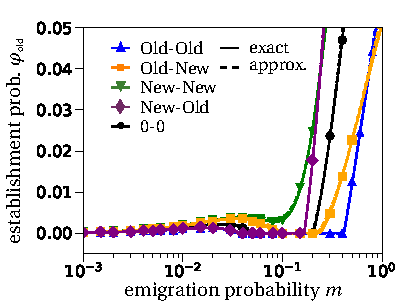
\includegraphics[width=\linewidth]{fig2a.pdf}
  		\caption{$\omega^\text{old}_m=1.35$ (large fecundity difference)}
	\end{subfigure}%
	\begin{subfigure}{.5\textwidth}
 		 \centering
 		 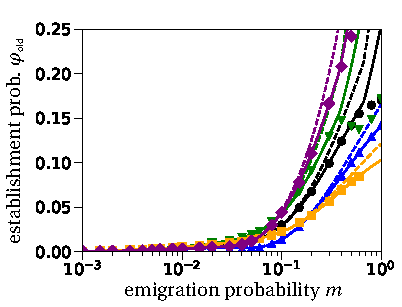
\includegraphics[width=\linewidth]{fig2c.pdf}
  	\caption{$\omega^\text{old}_m=1.45$ (small fecundity difference)}
	\end{subfigure}
	\begin{subfigure}{.5\textwidth}
  		\centering
  		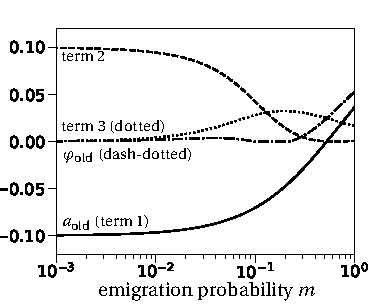
\includegraphics[width=\linewidth]{figS1c.pdf}
  		\caption{$\omega^\text{old}_m=1.35$ (large fecundity difference)}
	\end{subfigure}%
	\begin{subfigure}{.5\textwidth}
 		 \centering
 		 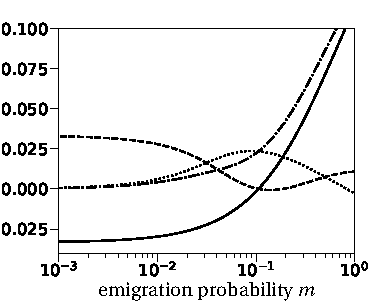
\includegraphics[width=\linewidth]{figS1d.pdf}
  	\caption{$\omega^\text{old}_m=1.45$ (small fecundity difference)}
	\end{subfigure}
	\caption{\textbf{Contribution of the different terms in eq.~\eqref{Seq:estab_approx} to the establishment probability $\varphi_{\text{old}}$.} Subfigures (a,b) are the same as Figs.~\ref{fig:vary_m_est}(a,c) in the main text. They show the establishment probability for a single mutant individual arising in an old-habitat patch for varying emigration probabilities $m$. In subfigures (c,d) we plot the terms from eq.~\eqref{Seq:estab_approx} separately ($\pi_w=0.5,\pi_m=-0.5$). Term 1, the mutant growth rate in old habitats (solid), increases with increasing dispersal rates as a consequence of relaxed competition. Term 2, the environmental effect (dashed), captures the differences between the growth rates in the habitats. The larger the difference, the larger its contribution to the overall establishment probability. Term 3, the effect of dispersal (dotted), (largely) increases with increasing dispersal rates $m$. The sum of the three terms is plotted as a dash-dotted line.}
	\label{Sfig:contribution}
\end{figure}

For clarity, we re-plot Figs.~\ref{fig:vary_m_est}(a,c) in Fig.~\ref{Sfig:contribution}(a,b), respectively. We try to explain the ongoing processes for each of the regions through the approximations of the establishment probabilities in eq.~\eqref{Seq:estab_approx}, see also Fig.~\ref{Sfig:contribution}(c,d). Note that these explanations are only valid for the establishment probability of a mutant initially in an old-habitat patch, $\varphi_{\text{old}}$. For the intuition behind the shape of $\varphi_{\text{new}}$ we refer to the corresponding section in the main text.

Region (i) is explained by the positive effect of dispersal. Mutants disperse from old- to new-habitat patches where they \chg{have a higher growth rate}. This effect is mediated through the third term of the establishment probability in eq.~\eqref{Seq:estab_approx}. \chg{Note that the first two terms of the approximation cancel out for small emigration probabilities $m$.}
While the third term increases with increasing emigration rate $m$, the second term in eq.~\eqref{Seq:estab_approx} decreases, cf. Fig.~\ref{Sfig:contribution}. 
In the formula this is mediated through \chg{the increase of the local growth rate in the old-habitat, $a_{\text{old}}$, i.e.\ it becomes less negative. Then both factors of the second term, $a_{\text{old}}$ and the difference $(a_{\text{old}}-a_{\text{new}})$, increase (which in turn decreases term two). The }\chg{intuitive} reason is that due to larger emigration probabilities $m$, more individuals leave old habitats before the reproductive event. This relaxes competition in these patches and therefore increases the local growth rate of mutants in old-habitat patches.   
%
%The intuition is that habitat differences become less important under stronger population mixing -- recall that the dispersal rate $m$ appears in the constant $C$ in the denominator. This alone would explain the decreasing curve of the second term. Additionally though, the local growth rate in old-habitat patches, $a_{\text{old}}$, is linked to the population demography which changes for varying $m$. With larger dispersal rates, more individuals leave the densely populated old habitats. This results in alleviated competition pressure for the remaining individuals, thus increasing the local growth rate $a_{\text{old}}$. This decreases the difference of growth rates $a_{\text{old}}-a_{\text{new}}$. Therefore, the local maximum can be explained by the decreasing environmental influence and the increasing dispersal effect, the second and the third term in eq.~\eqref{eq:estab_approx}, respectively. Hence, region (ii), beginning with the local maximum, is dominated by the decreasing effect of the environment on the establishment probability. 
Finally, in region (iii) dispersal is so large that the population homogenizes. This results in even less competitive pressure in old-habitat patches. Eventually, this yields a positive growth rate $a_{\text{old}}$ (first term in eq.~\eqref{Seq:estab_approx}). Therefore, this region is driven by the local growth rate in old habitats.

Note that region (iii) can be shifted to the left by increasing the absolute number of offspring of mutants in old-habitat patches, $\omega^\text{old}_m$, and therefore decreasing the local disadvantage of the mutant. If shifted sufficiently to the left, like in Fig.~\ref{Sfig:contribution}(d), region (ii) might vanish due to this effect.

\chg{Contrarily, if we set the fecundity parameter of the mutant in the old habitat to $\omega^\text{old}_m=1.1$, we see that region (iii) disappears for most dispersal schemes, cf. Fig.~\ref{Sfig:weak_fecundity}. Due to the low fecundity of the mutant, even under relaxed competition in old habitats, establishment of a mutant population is very unlikely. The final increase of our approximation in the dispersal schemes New-New and New-Old is due to our density-independence assumption in new habitats. For these large values of $m$ and the bias of the wild type towards new-habitat patches, this assumption is violated in the simulations explaining the deviation from the simulation results and our prediction. }

\begin{figure}
	\centering
	 	\begin{subfigure}{.5\textwidth}
  		\centering
  		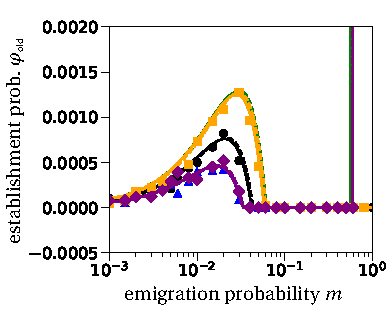
\includegraphics[width=\linewidth]{figS2a.pdf}
  		\caption{$\varphi_{\text{old}}$}
	\end{subfigure}%
	\begin{subfigure}{.5\textwidth}
 		 \centering
 		 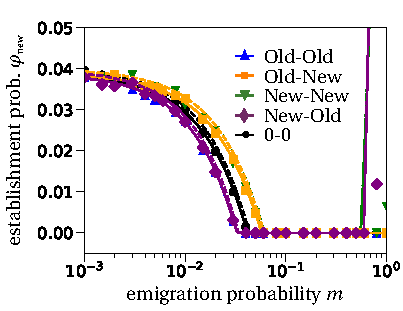
\includegraphics[width=\linewidth]{figS2b.pdf}
  	\caption{$\varphi_{\text{new}}$}
	\end{subfigure}
	\caption{\textbf{Disappearance of region (iii) for large fecundity differences in the old habitat.} If the mutant fecundity in old-habitat patches is too low, here $\omega^\text{old}_m=1.1$, the effect of relaxed competition is not strong enough to have an impact on the establishment probability for high dispersal rates. The establishment probability remains at zero.}
	\label{Sfig:weak_fecundity}
\end{figure}


%%%%%%%%%%%%%%%%%%%%%%%%%%%%%%%%%%%%%%%%%%%%%%%%%%%%%%%%%
% Native habitat type %%%%%%%%%%%%%%%%%%%%%%%%%%%%%%%%%%%
%%%%%%%%%%%%%%%%%%%%%%%%%%%%%%%%%%%%%%%%%%%%%%%%%%%%%%%%%
\newpage
\section{Habitat of origin of the adaptive mutation}
\chg{Here, we provide further insight into the origin of the adaptive mutation. Therefore we plot the establishment probabilities $\varphi_{\text{old}}$ and $\varphi_{\text{new}}$ when varying the frequency of old habitats, $f_{\text{old}}$. In Fig.~\ref{fig:origin} in the main text we have seen that most successful adaptive mutations arise in old-habitat patches. Here, we show that this is explained mostly due to the large mutational input that is provided by the much larger wild-type population sizes in old habitats, see Fig.~\ref{Sfig:vary_f_origin}(b). The establishment probability though is always larger for mutants that arise in new habitats than in old habitats (Fig.~\ref{Sfig:vary_f_origin}(a)). 
}

\begin{figure}[h!]
	\centering
	\begin{subfigure}{.5\textwidth}
  		\centering
  		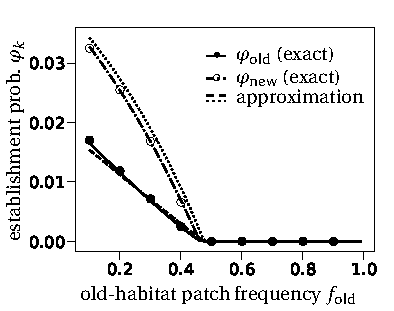
\includegraphics[width=\linewidth]{figS3a.pdf}
  		\caption{Establishment probabilities}
	\end{subfigure}%
	\begin{subfigure}{.5\textwidth}
 		 \centering
 		 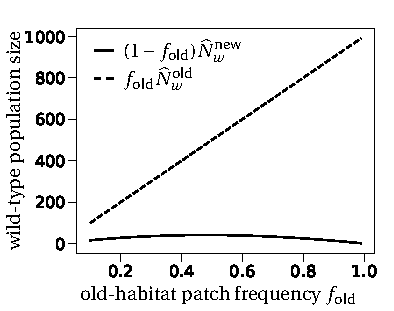
\includegraphics[width=\linewidth]{figS3b.pdf}
  	\caption{Stationary wild-type population size}
	\end{subfigure}
	\caption{\textbf{Establishment probability and stationary wild-type population size when varying the old-habitat frequency.} In the simulations we have used the standard set of parameters as given in Table~\ref{tab:parameters} and the unbiased dispersal scheme ($\pi_w=\pi_m=0$). In (a) we additionally chose the large fecundity difference scenario ($\omega^\text{old}_m=1.35$).}
	\label{Sfig:vary_f_origin}
\end{figure}

%Additionally, we investigate the habitat type of the origin of the adaptive mutations for low fecundity values of the mutant in the old habitat. While for large fecundity values of the mutant in the old habitat most successful lineages arise in the old habitat (Fig.~\ref{fig:origin} in the main text), we see that for lower fecundity values $\omega^\text{old}_m$ the contribution of new-habitat mutants approaches and occasionally exceeds the number of successful mutant lineages that emerge from old-habitat patches. In the subsequent figure, besides the default parameters as stated in Table 1 in the main text, we chose $\omega^\text{old}_m=1.05$ and $\theta = 10/(MK)$. The plot corresponding to Fig.~\ref{fig:origin} in the main text then looks as follows:

%\begin{figure}[h!]
%	\centering
%	\includegraphics[width=0.6\textwidth]{figS4.pdf}
%  	\caption{\textbf{Habitat type of the origin for strong fecundity differences in the old habitat ($\omega^\text{old}_m=1.05$).}}
%	\label{Sfig:origin}
%\end{figure}
\pete{There was a figure where the contribution from new habitats was larger than from old habitats. With the changed fecundities, I only get this behavior if the fecundity of the mutant is larger in the new patches than in the old patches, i.e. $\omega^\text{old}_m < a_{\text{new}}$. Also, for some reason the approximations do not work that well in these scenarios (I did not investigate why the estimated lines are bad -- soft sweeps still work fine but the other approximations don't.)}

%%%%%%%%%%%%%%%%%%%%%%%%%%%%%%%%%%%%%%%%%%%%%%%%%%%%%%%%%
% Large emigration rate %%%%%%%%%%%%%%%%%%%%%%%%%%%%%%%%%
%%%%%%%%%%%%%%%%%%%%%%%%%%%%%%%%%%%%%%%%%%%%%%%%%%%%%%%%%
\newpage
\section{Probability of establishment for large frequencies of old-habitat patches}
\chg{We plot the probability of establishment for a large frequency of old-habitat patches, $f_{\text{old}}$. As visible in Fig.~\ref{Sfig:vary_f} below, for high frequencies of old-habitat patches the probability of adaptation becomes very small, if not zero, for large emigration probabilities $m$. These high frequency of old-habitat patches are the patch configurations which mutants that were present before the first patch degrades, i.e. standing genetic variation mutants, experience. Therefore, it is very unlikely that the mutant, which will eventually rescue the population, was already present before the first degradation event.} This supports the explanation that homogenizing the population (large $m$) reduces the impact of standing genetic variation on the probability of evolutionary rescue, see Fig.~\ref{fig:sgv}(b) in the main text where $\pi_w=\pi_m=0$ was plotted.

\begin{figure}[h!]
	\centering
	\begin{subfigure}{.5\textwidth}
  		\centering
  		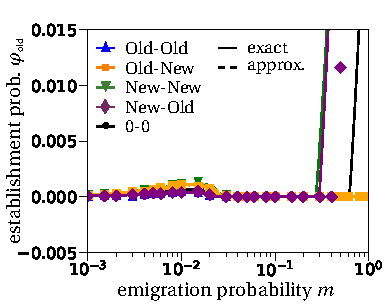
\includegraphics[width=\linewidth]{figS5a.pdf}
  		\caption{$\varphi_{\text{old}}$}
	\end{subfigure}%
	\begin{subfigure}{.5\textwidth}
 		 \centering
 		 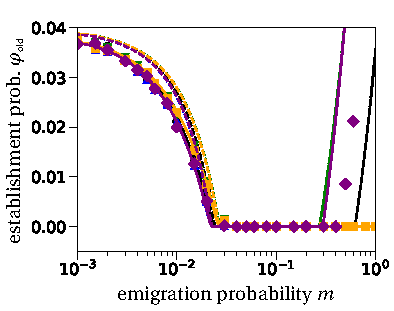
\includegraphics[width=\linewidth]{figS5b.pdf}
  	\caption{$\varphi_{\text{new}}$}
	\end{subfigure}
	\caption{\textbf{Probability of adaptation for a large frequency of old-habitat patches ($f_{\text{old}}=0.9$).} The fecundity of the mutant in old-habitat patches is set to $\omega^\text{old}_m=1.45$. Note also the difference between the scales of the y-axes in the two panels.}
	\label{Sfig:vary_f}
\end{figure}

%%%%%%%%%%%%%%%%%%%%%%%%%%%%%%%%%%%%%%%%%%%%%%%%%%%%%%%%%
% Comparison to pop gen %%%%%%%%%%%%%%%%%%%%%%%%%%%%%%%%%
%%%%%%%%%%%%%%%%%%%%%%%%%%%%%%%%%%%%%%%%%%%%%%%%%%%%%%%%%
\newpage
\section{Establishment probability in a model without demography}
Here, we consider a variation of our original model in order to investigate the impact of demography on the establishment probabilities $\varphi_{\text{old}}$ and $\varphi_{\text{new}}$. The dispersal process and the dynamics in old-habitat patches remain as studied before. In new-habitat patches we now assume that the population remains at carrying capacity, i.e. there is no longer a declining wild-type population. This means that the local growth rate $a_{\text{old}}$ in eq.~\eqref{Seq:s_old} takes the form for $\widehat{N}_w^{\text{new}}=K_{\text{new}}$. For simplicity we will also assume that $K_{\text{new}}=K_{\text{old}}=K$. In order to maintain the divergent selection assumption, we assume that the fecundity of the wild-type in the new habitat is below the fecundity of the mutant. %For simplicity, we assume that the fecundity values are given as
%\begin{equation}
%    \omega^\text{old}_w^{\text{old}} = \omega^\text{old}_m^{\text{new}} \quad \text{and} \quad \omega^\text{old}_w^{\text{new}} = \omega^\text{old}_m^{\text{old}}.
%\end{equation}
Therefore, we need to adjust the local growth rate of a single mutant, $a_{\text{new}}$. The local growth rate in old habitats, $a_{\text{old}}$, remains as outlined in eq.~\eqref{Seq:s_old}. We have
\begin{equation}
    1+a_{\text{new}} = K \frac{\omega^\text{old}_m^{\text{new}}}{\omega^\text{old}_w^{\text{new}} \widetilde{N}_w^{\text{new}}+ \omega^\text{old}_m^{\text{new}}}\approx K \frac{\omega^\text{old}_m^{\text{new}}}{\omega^\text{old}_w^{\text{new}} \widetilde{N}_w^{\text{new}}},
\end{equation}
which with the help of eq.~\eqref{Seq:wt_eq1} yields
\begin{equation}
    a_{\text{new}} \approx \frac{\omega^\text{old}_m^{\text{new}}}{\omega^\text{old}_w^{\text{new}}\left(1+\frac{m f_{\text{old}} (1-\widehat{\pi}_w)}{1-f_{\text{old}}+\widehat{\pi}_w f_{\text{old}}}\right)}.
\end{equation}

\chg{Note, that we again used that during the establishment phase the wild type is much more abundant than the mutant which explains the approximation in the two equations.}
Plugging this in the approximation of the establishment probability from eq.~\eqref{Seq:estab_approx} we find the curves in Fig.~\ref{Sfig:pop_gen}.

We see that, as briefly mentioned in the main text, region (iii) of the establishment probability disappears in these type of models except for the Old-New and the New-Old dispersal schemes. The reason for the disappearance of the region is that relaxed competition only plays a subordinate role for the symmetric dispersal schemes (Old-Old, New-New and 0-0). In other words, these dispersal schemes maintain the local frequencies of the mutant at the same level as before the dispersal step and by that do not change the population dynamics. In contrast, the Old-New dispersal scheme strongly increases the frequency of mutants in new-habitat patches and by that increases the establishment probability. It is worth mentioning though, that this is not an effect of relaxed competition but rather a biased dispersal of the mutant into the habitat where it is favored. Solely for the New-Old dispersal scheme where individuals prefer the habitat they are relatively less fit, we see a relaxed competition scenario in old-habitat patches. For high dispersal rates $m$ the majority of the wild-type individuals emigrate to new habitats and by that leave space for the rare mutants in old-habitat patches to reproduce. This explains why this dispersal scheme still shows the characteristic pattern of a three-stage establishment probability.   \newpage 

\begin{figure}[h!]
	\centering
	\begin{subfigure}{.5\textwidth}
  		\centering
  		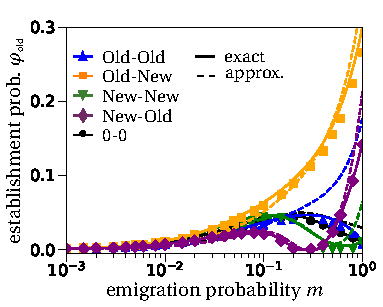
\includegraphics[width=\linewidth]{figS6a.pdf}
  		\caption{$\varphi_{\text{old}}$ with $\omega^\text{old}_m=1.35$ (large fecundity difference)}
	\end{subfigure}%
	\begin{subfigure}{.5\textwidth}
 		 \centering
 		 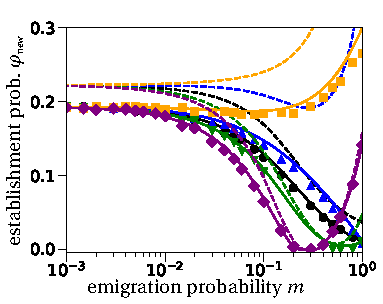
\includegraphics[width=\linewidth]{figS6b.pdf}
  	\caption{$\varphi_{\text{new}}$ with $\omega^\text{old}_m=1.35$}
	\end{subfigure}
	\begin{subfigure}{.5\textwidth}
  		\centering
  		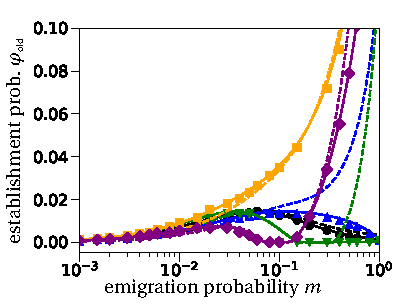
\includegraphics[width=\linewidth]{figS6c.pdf}
  		\caption{$\varphi_{\text{old}}$ with $\omega^\text{old}_m=1.45$ (small fecundity difference)}
	\end{subfigure}%
	\begin{subfigure}{.5\textwidth}
 		 \centering
 		 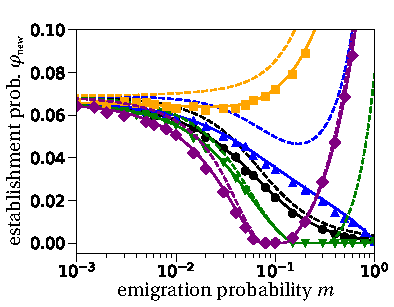
\includegraphics[width=\linewidth]{figS6d.pdf}
  	\caption{$\varphi_{\text{new}}$ with $\omega^\text{old}_m=1.45$}
	\end{subfigure}
  	\caption{\textbf{Establishment probability when populations in both habitats are at carrying capacity.} We plot the establishment probability for a single mutant either initially in an old-habitat patch (a,c) or in a new-habitat patch (b,d). The numerical solution (solid lines) still approximates the simulated data reasonably well. The analytical approximation (dashed lines) however deviates strongly from the data due to large growth rates ($a_{\text{new}}\approx 0.2$) so that the conditions for the approximation to hold are violated. In this case, in eq.~\eqref{Seq:estab_approx} higher order corrections would need to be taken into account. \chg{The fecundity values in the new habitat are given by $\omega^\text{old}_w^{\text{new}} = \omega^\text{old}_m^{\text{old}}$ and $\omega^\text{old}_m^{\text{new}} = \omega^\text{old}_w^{\text{old}}$ and the carrying capacity is $K_{\text{new}}=K_{\text{old}}=K=500$.} Missing data points (mostly for the negative density-dependent dispersal scheme -- green triangles) are explained by too large computation times. All data points are averages from $10^4$ independent runs. Note the varying y-axes scales.}
	\label{Sfig:pop_gen}
\end{figure}


%%%%%%%%%%%%%%%%%%%%%%%%%%%%%%%%%%%%%%%%%%%%%%%%%%%%%%%%%
% Origin dispersal schemes %%%%%%%%%%%%%%%%%%%%%%%%%%%%%%
%%%%%%%%%%%%%%%%%%%%%%%%%%%%%%%%%%%%%%%%%%%%%%%%%%%%%%%%%
\newpage
\section{Habitat of origin dependent on the dispersal scheme}
The habitat type of the origin of the rescue mutation is largely independent of the considered dispersal scheme. For $\omega^\text{old}_m=1.35$ we have plotted the relative contribution of each natal habitat type to the probability of evolutionary rescue, Fig.~\ref{Sfig:natal_habitat}. We do not see large differences between the three symmetric dispersal schemes (0-0, Old-Old, and New-New) and the Old-New dispersal scheme. \chg{Only for the New-Old dispersal schemes we see an increase in the contribution of mutants emerging from old-habitat patches for very high emigration probabilities $m$. A possible explanation is the large probability of establishment for a mutant emerging in old-habitat patches for this parameter set (cf. Fig.~\ref{Sfig:contribution}(a)).}

\begin{figure}[h!]
	\centering
	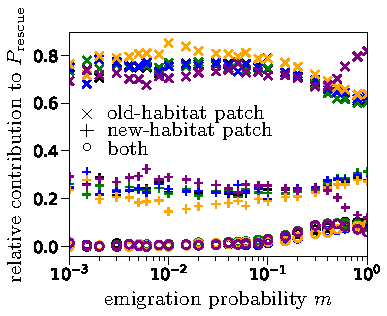
\includegraphics[width=0.6\textwidth]{figS7.pdf}
  	\caption{\textbf{Habitat type of the origin of the rescue mutant dependent on the dispersal scheme.} Varying the emigration probability $m$ we plot the relative contributions of each habitat type to the probability of evolutionary rescue. The color-coding is as in the main text: black for 0-0, blue for the Old-Old, green for the New-New, orange for the Old-New, and purple for the New-Old dispersal scheme.}
	\label{Sfig:natal_habitat}
\end{figure}

%%%%%%%%%%%%%%%%%%%%%%%%%%%%%%%%%%%%%%%%%%%%%%%%%%%%%%%%%
% Bibliography %%%%%%%%%%%%%%%%%%%%%%%%%%%%%%%%%%%%%%%%%%
%%%%%%%%%%%%%%%%%%%%%%%%%%%%%%%%%%%%%%%%%%%%%%%%%%%%%%%%%
\newpage
\bibliographystyle{plainnat}
\bibliography{dispersal.bib}

\end{document}